% This is samplepaper.tex, a sample chapter demonstrating the
% LLNCS macro package for Springer Computer Science proceedings;
% Version 2.21 of 2022/01/12
%
\documentclass[runningheads]{llncs}
%
\usepackage[T1]{fontenc}
% T1 fonts will be used to generate the final print and online PDFs,
% so please use T1 fonts in your manuscript whenever possible.
% Other font encondings may result in incorrect characters.
%
\usepackage{graphicx}
% Used for displaying a sample figure. If possible, figure files should
% be included in EPS format.
%
% If you use the hyperref package, please uncomment the following two lines
% to display URLs in blue roman font according to Springer's eBook style:
%\usepackage{color}
%\renewcommand\UrlFont{\color{blue}\rmfamily}
%\urlstyle{rm}
%
% Packages required for listing Lean code
\usepackage[T1]{fontenc}
\usepackage[utf8]{inputenc}
\usepackage{listings}
\usepackage{color}
\def\lstlanguagefiles{lstlean.tex}
\definecolor{hypcolor}{rgb}{0.85, 0.48, 0.0}
\lstdefinestyle{leanHH}{
  language=lean,
  moredelim=**[is][\color{hypcolor}]{|!}{!|},
}
\usepackage{amssymb}
\newsavebox\vEq
\newsavebox\vmap
\newsavebox\vrev
\newsavebox\vmaprev
\newsavebox\vrevrev
%\definecolor{keywordcolor}{rgb}{0.7, 0.1, 0.1}   % red
\definecolor{keywordcolor}{rgb}{0.0, 0.0, 0.0}   % black
\definecolor{tacticcolor}{rgb}{0.0, 0.3, 0.8}    % blue
\definecolor{commentcolor}{rgb}{0.4, 0.4, 0.4}   % grey
%\definecolor{symbolcolor}{rgb}{0.0, 0.1, 0.6}    % blue
\definecolor{symbolcolor}{rgb}{0.0, 0.0, 0.0}    % black
%\definecolor{sortcolor}{rgb}{0.1, 0.5, 0.1}      % green
\definecolor{sortcolor}{rgb}{0.0, 0.0, 0.0}      % black
\definecolor{attributecolor}{rgb}{0.7, 0.1, 0.1} % red

\usepackage{fancybox}
\makeatletter
\newenvironment{CenteredBox}{% 
\begin{Sbox}}{% Save the content in a box
\end{Sbox}\centerline{\parbox{\wd\@Sbox}{\TheSbox}}}% And output it centered
\makeatother

\usepackage{amsmath}
\usepackage{algorithm2e}
\SetKwProg{Fn}{Function}{}{end}
\SetKwSwitch{Switch}{Case}{Other}{match}{}{case}{otherwise}{}{}
\SetKwFor{For}{for}{do}{}
\SetKwInOut{Input}{In}
\SetKwInOut{Output}{Out}
\SetKw{Continue}{continue}
\SetKw{Break}{break}

\newcommand{\vnewname}{\ensuremath{\mathit{newname}}\xspace}
\newcommand{\vlf}{\ensuremath{\mathit{lf}}\xspace}
\newcommand{\vlvar}{\ensuremath{\mathit{lvar}}\xspace}
\newcommand{\vargs}{\ensuremath{\mathit{args}}\xspace}
\newcommand{\vlargs}{\ensuremath{\mathit{largs}}\xspace}
\newcommand{\vatype}{\ensuremath{\mathit{atype}}\xspace}
\newcommand{\vaabst}{\ensuremath{\mathit{aabst}}\xspace}
\newcommand{\vbabst}{\ensuremath{\mathit{babst}}\xspace}
\newcommand{\vmatches}{\ensuremath{\mathit{matches}}\xspace}
\newcommand{\vmaxInsts}{\ensuremath{\mathit{maxInsts}}\xspace}
\newcommand{\vhi}{\ensuremath{\mathit{hi}}\xspace}
\newcommand{\vci}{\ensuremath{\mathit{ci}}\xspace}
\newcommand{\vactiveci}{\ensuremath{\mathit{activeci}}\xspace}
\newcommand{\vnewci}{\ensuremath{\mathit{newci}}\xspace}
\newcommand{\vprevhi}{\ensuremath{\mathit{prevhi}}\xspace}
\newcommand{\vnewhi}{\ensuremath{\mathit{newhi}}\xspace}
\newcommand{\vmonohi}{\ensuremath{\mathit{monohi}}\xspace}
\newcommand{\vnh}{\ensuremath{\mathit{nh}}\xspace}
\newcommand{\vnc}{\ensuremath{\mathit{nc}}\xspace}

\begin{document}

\title{Lean-auto: An interface between Lean4 and Automated Theorem Provers}
%
%\titlerunning{Abbreviated paper title}
% If the paper title is too long for the running head, you can set
% an abbreviated paper title here
%
\author{
  Yicheng Qian\inst{3}{ % TODO: \orcidID{}
  } \and
  Joshua Clune\inst{1}\orcidID{0000-0003-4047-6196} \and
  Jasmin Blanchette\inst{2}\orcidID{0000-0002-8367-0936} \and
  Clark Barrett\inst{3}\orcidID{0000-0002-9522-3084} \and
  Jeremy Avigad\inst{1}\orcidID{0000-0003-1275-315\textrm{X}} \\
  % TODO: To be determined
}
%
\authorrunning{Y. Qian et al.}
% First names are abbreviated in the running head.
% If there are more than two authors, 'et al.' is used.
%
\institute{
  Carnegie Mellon University, Pittsburgh, PA 15213, USA \and
  Heinrich-Heine-Universität Düsseldorf, 40225 Düsseldorf, Germany \and
  Stanford University, Stanford, CA 94305, USA
}
%
\maketitle              % typeset the header of the contribution
\begin{abstract}
  Proof automation is crucial to large-scale formal mathematics and software/hardware verification projects
  in ITPs. Sophisticated tools called Hammers have been developed to provide general proof
  automation in ITPs such as Coq and Isabelle, leveraging the power of ATPs. An important
  component of Hammers is the translation algorithm from the ITP's logical system
  to the ATP's logical system. In this paper, we propose a novel translation algorithm
  for ITPs based on dependent type theory. The algorithm is implemented in Lean4 under
  the name Lean-auto. The core of our algorithm is an extension of
  the monomorphization procedure implemented in Isabelle Sledgehammer.
  Soundness is guaranteed, and experimental results suggest that
  the algorithm is sufficiently complete for practical uses of Lean in formal mathematics and
  software verification. We also show that our algorithm produces more efficient
  translations compared to the encoding-based approach used in CoqHammer.
  
  \keywords{Proof Automation \and Lean \and Dependent Type Theory}
\end{abstract}
\section{Introduction}

  Interactive Theorem Provers (ITPs) \cite{Harrison2014HistoryOI}
  are widely used in formal mathematics and software/hardware verification. Hammers
  \cite{Blanchette2016HammeringTQ}\cite{Czajka2018HammerFC} are type of proof automation tool for
  ITPs which utilize Automated Theorem Provers (ATPs, including SMT solvers).
  When using ITPs, a significant amount of straightforward but tedious proof tasks
  tasks arise from the proof development process, which requires huge amounts of human
  effort to complete. Hammers have proved useful in solving these proof tasks automatically \cite{Paulson2012ThreeYO}.
  
  A hammer has three main components: premise selection, translation from ITP to
  ATP, and proof reconstruction from ATP to ITP. Premise selection collects
  the necessary information needed to solve a proof task, translation exports
  the collected information from the ITP to the ATP, and proof reconstruction imports the
  proof returned by the ATP to the ITP. The discrepancies between logical systems of ATPs and ITPs pose
  significant challenges to translation procedures between them.
  Several popular ITPs are based on highly expressive logical systems.
  For example, Isabelle \cite{Isabelle} is based on polymorphic higher-order logic, while
  Coq \cite{CoqRefMan}, Lean4 \cite{Lean4} and Agda \cite{Agda}
  are based an even more expressive logical system called dependent type
  theory\footnote{Or \textit{calculus of inductive constructions (CIC)}, depending
  on whether inductive type is considered as an extension.}
  \cite{LambdaWithType}\cite{Coquand1988}.
  Moreover, features such as typeclasses \cite{TypeClassHaskell}, universe polymorphism \cite{UPolyCoq} and inductive types \cite{CICIndDef}
  are commonly used as extensions to the base logical system to enhance usability of the ITP.
  On the other hand, ATPs are usually based on less expressive logical systems such
  as first-order logic (FOL) \cite{CVC5}\cite{Vampire}\cite{Z3Paper}\cite{EProver} and
  higher-order logic (HOL) \cite{HOVampire}\cite{ZipperpositionMakeWork}\cite{HOEProver}.
  An overview of the logical systems relevant to our work will be given in sect. \ref{sublogsys}.

  The focus of our paper is the Lean to ATP translation procedure in Lean-auto.
  However, Lean-auto does have a proof reconstruction procedure which fully supports proof
  reconstruction of one of the three types of ATPs we use to evaluate Lean-auto.
  Ongoing projects are expected to implement premise selection and more proof reconstruction support.
  See sect. \ref{sectexpr} for more discussions.

  There are two existing approaches for translation from more expressive
  logical systems to less expressive ones: encoding-based translation and monomorphization.
  Encoding-based translation is used in CoqHammer \cite{Czajka2018HammerFC}
  to translate Coq into untyped FOL. Monomorphization is used to
  eliminate polymorphism in Isabelle Sledgehammer \cite{Blanchette2016HammeringTQ}\cite{Paulson2012ThreeYO}.
  We found that encoding-based translation tends to produce large translation outputs
  on complex problems arising from real ITP use cases, which negatively affects the performance of ATPs.
  Therefore, we decided to use monomorphization in Lean-auto. An overview of these two
  translation methods and related discussions will be given in sect. \ref{subencmon}.

  Since ATPs have started supporting HOL in recent years \cite{HOVampire}\cite{ZipperpositionMakeWork}\cite{HOEProver},
  we decided that Lean-auto should translate Lean4 to HOL. The overall translation has
  two stages: preprocessing (sect. \ref{sectprep}) and monomorphization.
  Monomorphization itself has three stages: quantifier instantiation (sect. \ref{sectinst}),
  $\lambda_\to^*$ abstraction (sect. \ref{sectabst}) and universe lifting. Preprocessing translates Lean4
  into dependent type theory, and monomorphization translates dependent type theory
  into HOL. The monomorphization procedure is inspired by Isabelle Sledgehammer.
  However, since Isabelle is based on HOL, which is considerably different from
  dependent type theory, the algorithm is thoroughly redesigned.
\section{Motivating Examples} \label{motex}

\begin{lrbox}{\vEq} {\color{hypcolor} \verb|Eq|} \end{lrbox}
\begin{lrbox}{\vmap} {\color{hypcolor} \verb|map|} \end{lrbox}
\begin{lrbox}{\vrev} {\color{hypcolor} \verb|reverse|} \end{lrbox}
\begin{lrbox}{\vmaprev} {\color{hypcolor} \verb|map_reverse|} \end{lrbox}
\begin{lrbox}{\vrevrev} {\color{hypcolor} \verb|reverse_reverse|} \end{lrbox}

In section \ref{exabst} and \ref{exinst}, we will demonstrate the execution of our monomorphization procedure on a
concrete example. Note that both the examples and the monomorphization procedure
here are simplified. Sect. \ref{exqdet} contains discussions and more examples
to illustrate details of our monomorphization procedure.

\subsection{$\lambda_\to^*$ Abstraction} \label{exabst}

\begin{figure}
  \begin{CenteredBox}
    \lstinputlisting[style=leanHH]{LeanCode/reverse_map_pretty.inp}
  \end{CenteredBox}
  \caption{Lean4 proof state of a problem involving \textbf{List}} \label{leanlistpretty}
\end{figure}

The Lean4 proof state of the problem we will consider is shown in Figure \ref{leanlistpretty}.
The hypotheses are displayed before $\vdash$, while the goal comes after $\vdash$.
\usebox{\vmaprev} states that \usebox{\vmap} commutes with \usebox{\vrev}, and
\usebox{\vrevrev} states that \usebox{\vrev} is the inverse function of itself.
We will focus on the most important part of monomorphization, which is the
$\lambda C$ to $\text{HOL}^*$ translation. Note that the problem is already in the
$\lambda C$ fragment of Lean.

\begin{figure}
  \begin{CenteredBox}
    \lstinputlisting[style=leanHH]{LeanCode/reverse_map_explicit.inp}
  \end{CenteredBox}
  \caption{Lean4 proof state after quantifier introduction and proof by contradiction, with implicit arguments displayed.
    Note that the equality sign in figure \ref{leanlistpretty} is a syntactic sugar of
    the polymorphic function {\usebox{\vEq}} seen here}
  \label{leanlistexplicit}
\end{figure}

As a standard first step, we introduce all the $\forall$ quantifiers
of the goal into the context, and apply proof by contradiction. The resulting proof state
is shown in Figure \ref{leanlistexplicit}.
For clarity, we have displayed the implicit arguments of all the functions.

First, we focus on translating \texttt{neg\_goal} into $\text{HOL}^*$. Following the
discussion of sect. \ref{subencmon}, we would like to find an $\text{HOL}^*$ formula $\varphi$
and a ``substitution'' $\sigma$ such that the image of $\varphi$ under $\sigma$ is \texttt{neg\_goal}.
Features not allowed in $\varphi$ include polymorphic. We also want the problem to
be provable after the translation, so $\varphi$ should preserve as much information in
\texttt{neg\_goal} as possible.

Three polymorphic functions, namely \usebox{\vEq}, \usebox{\vmap} and \usebox{\vrev}, occur in the \texttt{neg\_goal}.
Although these functions are polymorphic, instances of these functions
with dependent arguments instantiated could behave like monomorphic functions.
The type constructor \texttt{List} is also not allowed in $\text{HOL}^*$, but
\texttt{List A} and \texttt{List B} behave just like $\text{HOL}^*$ type variables.
Therefore, we can choose
$$\begin{aligned}
\varphi := & \ \neg (\mathsf{EqLB} \ (\mathsf{rB} \ (\mathsf{mAB} \ f^* \ (\mathsf{rA} \ \mathit{xs}^*))) \ (\mathsf{mAB} \ f^* \ \mathit{xs}^*)) \\
\sigma := & \ \{\mathsf{EqLB} \mapsto \texttt{@Eq (List B)}, \ \ \mathsf{mAB} \mapsto \texttt{@map A B}, \\
          & \ \ \mathsf{rA} \mapsto \texttt{@reverse A}, \ \ \mathsf{rB} \mapsto \texttt{@reverse B}, \ \ f^* \mapsto \texttt{f}, \ \ \mathit{xs}^* \mapsto \texttt{xs}\}
\end{aligned}$$

In a sense, the monomorphic instances of polymorphic functions are ``abstracted'' to $\text{HOL}^*$
variables. Note that the logical rules of $\text{HOL}^*$ are not relevant to this abstraction procedure, only
the term calculus $\lambda_\to^*$ is involved. Therefore, we name this procedure $\lambda_\to^*$ \textit{abstraction}.

However, $\lambda_\to^*$ abstraction is not directly applicable to \usebox{\vmaprev} and
\usebox{\vrevrev}, because dependent arguments of polymorphic functions in them are universally
quantified. Naturally, we would like to instantiate these quantifiers to make $\lambda_\to^*$
abstraction applicable.

\subsection{Quantifier Instantiation} \label{exinst}

If we were to prove the goal manually, there are at least two ways we can proceed. We can
either first use \texttt{@map\_reverse A B} to swap the outer \texttt{reverse} with \texttt{map}, then
use \texttt{@reverse\_reverse A} to eliminate \texttt{reverse}; or, first use
\texttt{@map\_reverse A B} to swap the inner \texttt{reverse} with \texttt{map}, then
use \texttt{@reverse\_reverse B} to eliminate \texttt{reverse}. Notice how quantifiers
in the hypotheses are instantiated so that the dependent arguments of polymorphic functions
in the instantiated hypotheses match the dependent arguments of their monomorphic instances in the goal.

Quantifier instantiation in Lean-auto's monomorphization procedure is based
on a matching procedure that reflects the above observation. Given a set of formulas $S$,
the matching procedure first computes the set $M$ of monomorphic instances of polymorphic functions occurring
in $S$, then matches type-quantified formulas in $S$ with elements of $M$. For example,
given $S=$\texttt{\{@map\_reverse, @reverse\_reverse, neg\_goal\}}, the set $M$ will be
\texttt{\{@reverse A, @reverse B, @map A B, @Eq (List B)\}}, all of which collected from \texttt{neg\_goal}.
The matching procedure will preform the following matchings:

\begin{enumerate}
  \item \texttt{@Eq (List $\beta$)} in \usebox{\vmaprev} with \texttt{@Eq (List B)},
    which produces \texttt{fun $\alpha$ => @map\_reverse $\alpha$ B}
  \item \texttt{@map $\alpha$ $\beta$} in \usebox{\vmaprev} with \texttt{@map A B},
    which produces \texttt{map\_reverse A B}
  \item \texttt{@reverse $\alpha$} in \usebox{\vmaprev} with \texttt{@reverse A} and \texttt{@reverse B},
    which produces \texttt{@map\_reverse A} and \texttt{@map\_reverse B}
  \item \texttt{@reverse $\beta$} in \usebox{\vmaprev} with \texttt{@reverse A} and \texttt{@reverse B},
    which produces \texttt{fun $\alpha$ => @map\_reverse $\alpha$ A} and \texttt{fun $\alpha$ => @map\_reverse $\alpha$ B}
  \item \texttt{@Eq (List $\alpha$)} in \usebox{\vrevrev} with \texttt{@Eq (List B)},
    which produces \texttt{@reverse\_reverse B}
  \item \texttt{@reverse $\alpha$} in \usebox{\vrevrev} with \texttt{@reverse A} and \texttt{@reverse B},
    which produces \texttt{@reverse\_reverse A} and \texttt{@reverse\_reverse B}
\end{enumerate}

Since \texttt{@reverse\_reverse A}, \texttt{@reverse\_reverse B} and \texttt{@map\_reverse A B}
are present, the instances produced are already sufficient for proving the goal.
But generally speaking, the newly generated hypothesis instances and polymorphic function instances
in them can still be matched with each other (and existing instances) to produce new useful results.
% TODO: Give a concrete example taken from my graduation thesis?
Hence, the monomorphization procedure in Lean-auto uses a saturation loop which
repeats the matching procedure until either no new instances can be produced or a predefined
threshold is reached.

\subsection{The requirement of $\lambda_\to^*$ abstraction on quantifier instantiation} \label{exqdet}

\begin{figure}
  \begin{CenteredBox}
    \begin{lstlisting}[style=leanHH]
|!@DFunLike.coe!| : {F : Type (max u_1 u_5)}
  → {α : outParam (Type u_1)} → {β : outParam (α → Type u_5)}
  → [self : DFunLike F α β] → F → (a : α) → β a

@DFunLike.coe (A₀ →+ B₀) A₀ (fun x => B₀) AddMonoidHom.instFunLike f₀ a 
    \end{lstlisting}
  \end{CenteredBox}
  \caption{The function \texttt{DFunLike.coe} from MathLib4 and an expression
  containing it}
  \label{dfun}
\end{figure}

Note that whether an argument is dependent depends on how previous arguments
are instantiated. Consider the example shown in figure \ref{dfun}. The return
type \texttt{$\beta$ a} depends on the last argument \texttt{a : $\alpha$} in the signature of
\texttt{DFunLike.coe}. However, when $\beta$ is instantiated with \texttt{fun x => B$_0$}, as in the
expression at the bottom of figure \ref{dfun}, the return type \texttt{$\beta$ a} reduces to \texttt{B$_0$},
which no longer depends on the last argument. Lean-auto takes preceding arguments into
consideration when determining whether an argument is dependent, and is able to detect
that the last argument is non-dependent in this case.
\section{$\lambda_\to^*$ abstraction}\label{sectabst}

\subsection{$\lambda C$, $\lambda_\to^*$ and $\lambda_\to$}

In this subsection, we define three type systems: $\lambda C, \lambda_\to^*$ and $\lambda_\to$. $\lambda C$
is calculus of constructions with a countable family of non-cumulative universe levels, similar
to the type theory of Lean; $\lambda_\to^*$ is simply typed lambda calculus with a countable
family of universe levels, without $\mathsf{U}_0$ and without the typing relation
$\mathsf{U}_\ell : \mathsf{U}_{\ell + 1}$, intended to model the output of Lean-auto's translation;
$\lambda_\to$ is simply typed lambda calculus. All three systems will be
specified as pure-type systems $(\mathcal{S}, \mathcal{A}, \mathcal{R})$, where $\mathcal{S}$
is the set of sorts, $\mathcal{A} \subseteq \mathcal{S}^2$ is the set of axioms, and
$\mathcal{R} \subseteq \mathcal{S}^3$ corresponds to the formation rules. The syntactical
equality of terms will be denoted as $=$, and the $\beta\eta$-equivalence of terms will be
denoted as $\cong$.

\begin{definition} $\lambda C$ is the pure type system $(\mathcal{S}, \mathcal{A}, \mathcal{R})$ where
  $$\mathcal{S} := \{\mathsf{U}_\ell | \ell \in \mathbb{N}\} \ \ \ \mathcal{A} := \{(\mathsf{U}_\ell, \mathsf{U}_{\ell + 1}) | \ell \in \mathbb{N}\}$$
  $$\mathcal{R} := \{(\mathsf{U}_\ell, \mathsf{U}_m, \mathsf{U}_{\mathsf{imax}(\ell, m)}) | \ell \in \mathbb{N}, m \in \mathbb{N}\}$$
  $$\mathsf{imax}(m, n) := \left\{\begin{aligned}
    \mathsf{max}(m, n), & & n > 0 \\
    0, & & n = 0
  \end{aligned}\right.$$

  The set of $\lambda_C$ terms will be denoted as $\mathcal{T}_C$.
\end{definition}

\begin{definition} $\lambda_\to^*$ is the pure type system $(\mathcal{S}, \mathcal{A}, \mathcal{R})$ where
  $$\mathcal{S} := \{\mathsf{U}_\ell | \ell \in \mathbb{N}^*\} \cup \{\mathsf{U}_\ell' | \ell \in \mathbb{N}^*\} \ \ \
    \mathcal{A} := \{(\mathsf{U}_\ell, \mathsf{U}_\ell') | \ell \in \mathbb{N}^*\}$$
  $$\mathcal{R} := \{(\mathsf{U}_\ell, \mathsf{U}_m, \mathsf{U}_{\mathsf{max} \{l, m\}}) | \ell \in \mathbb{N}^*, m \in \mathbb{N}^*\}$$

  The set of $\lambda_\to^*$ terms will be denoted as $\mathcal{T}_\to^*$.
\end{definition}

\begin{definition} $\lambda_\to$ is the pure type system $(\mathcal{S}, \mathcal{A}, \mathcal{R})$ where
  $$\mathcal{S} := \{\mathsf{U}_1, \mathsf{U}_1'\} \ \ \ \mathcal{A} := \{(\mathsf{U}_1, \mathsf{U}_1')\} \ \ \ 
    \mathcal{R} := \{(\mathsf{U}_1, \mathsf{U}_1, \mathsf{U}_1)\}$$
  This is equivalent to simply typed lambda calculus, where $\mathsf{U}_1$ and $\mathsf{U}_1'$ are
  usually denoted as $*$ and $\square$, respectively. The set of $\lambda_\to$ terms will be denoted
  as $\mathcal{T}_\to$.
\end{definition}

\begin{theorem} A $\lambda_\to^*$ problem is provable iff it is $\lambda_\to$ provable after forgetting
  universe levels, assuming the existence of lifting functions in $\lambda C$.
\end{theorem}
\begin{proof} \textbf{TODO}
  (Put this after the definition of provability)
  (Maybe a direct induction would be more elegant?)
  If a $\lambda_\to^*$ problem is provable, obviously it is $\lambda_\to$ provable
  after forgetting the universe levels. If a $\lambda_\to^*$ problem is $\lambda_\to$ provable
  after forgetting the universe levels, note that the lifting of a $\lambda_\to^*$ problem is sort of
  an instance of the problem after forgetting universe levels, hence provable. Moreover,
  a $\lambda_\to^*$ problem is provable iff its lifting is provable.  
\end{proof}

\subsection{Essentially higher-order problem}

\begin{definition} Let $\sigma : V \to \mathcal{T}_C$ be a mapping.
  Define its extension $\overline{\sigma} : \mathcal{T}_C \to \mathcal{T}_C$ as
  $$\overline{\sigma}(\mathsf{U}_\ell) := \mathsf{U}_\ell$$
  $$\overline{\sigma}(x) := \sigma(x), \text{ for }x \in V$$
  $$\overline{\sigma}(M \ N) := \overline{\sigma}(M) \ \overline{\sigma}(M)$$
  $$\overline{\sigma}(\lambda x : s. M) := \lambda x : \overline{\sigma}(s). \overline{\sigma[x \mapsto x]}(M)$$
  $$\overline{\sigma}(\forall x : s. M) := \forall x : \overline{\sigma}(s). \overline{\sigma[x \mapsto x]}(M)$$
  where
  $$\sigma[u \to t](x) := \left\{\begin{aligned}
    & t & & x = u \\
    & \sigma(x) & & x \in V \backslash \{u\}
  \end{aligned}\right.$$
\end{definition}

\begin{definition} A substitution is a triple $(\Gamma, \Gamma', \sigma)$ where $\Gamma, \Gamma'$ are $\lambda C$ contexts
  and $\sigma : V \to \mathcal{T}_C$, such that for all $(u : \tau) \in \Gamma$,
  $$\Gamma' \vdash \sigma(u) : \overline{\sigma}(\tau)$$
  $\Gamma$ is called the domain of the substitution, and $\Gamma'$ is called the codomain of the substitution.
\end{definition}

\begin{theorem}
  Let $(\Gamma, \Gamma', \sigma)$ be a substitution. If $\Gamma \vdash t : s$, then $\Gamma' \vdash \overline{\sigma}(t) : \overline{\sigma}(s)$
\end{theorem}
\begin{proof} Induction on the derivation of $\Gamma \vdash t : s$, note that $\Gamma'$ and $\sigma$
  should be universally quantified in the induction hypothesis.
\end{proof}

\begin{definition} Let $\Gamma$ be a $\lambda C$ context and $t_1, t_2$ be $\lambda C$ terms.
  If variable set $M$ and substitution $(\Gamma, \Gamma', \sigma)$ satisfies
  \begin{enumerate}
    \item There exists a $\lambda C$ term $s$ such that $\Gamma' \vdash \overline{\sigma}(t_1) : s$ and $\Gamma' \vdash \overline{\sigma}(t_2) : s$
    \item $\overline{\sigma}(t_1) \cong \overline{\sigma}(t_2)$
    \item For all variables $v \in \Gamma \backslash M$, $\sigma(v) = v$
  \end{enumerate}
  Then $(\Gamma, \Gamma', \sigma)$ is called a $M$-unifier of $t_1$ and $t_2$. In the context of Lean,
  this corresponds to a unifier of $t_1$ and $t_2$ under context $\Gamma$, with $M$ as the set of metavariables.
\end{definition}

\begin{definition} Many-sorted higher-order logic (HOL) is defined as $\lambda_\to^*$ augmented
  with the following symbols:
  \begin{enumerate}
    \item $\mathsf{Bool}$
    \item $\bot'$ and $\to'$
    \item $\forall'_t$, for each $t \in \mathcal{T}_\to^*$
  \end{enumerate}
  
  \noindent and the following derivation rules:
  $$\frac{}{\vdash \mathsf{Bool} : \mathsf{U}_1} \ \ \ \ \frac{}{\Gamma \vdash \bot' : \mathsf{Bool}}$$
  $$\frac{}{\Gamma \vdash \to' : \mathsf{Bool} \to \mathsf{Bool} \to \mathsf{Bool}} \ \ \ \
  \frac{\Gamma \vdash s : \mathsf{U}_\ell}{\Gamma \vdash \forall'_s : (s \to \mathsf{Bool}) \to \mathsf{Bool}}$$
  
  \noindent For simplicity, we use $\forall' (x : \alpha), t$ as a shorthand for $\forall'_\alpha \ (\lambda x : \alpha. t)$

  The canonical embedding $\pi : \mathcal{T}_\to^* \to \mathcal{T}_C$ of HOL into $\lambda C$ is defined as follows:
  $$\pi(\mathsf{Bool}) := \mathsf{U}_0 \ \ \ \pi(\mathsf{U}_\ell) := \mathsf{U}_\ell \ \ \
    \pi(\mathsf{U}_\ell') := \mathsf{U}_{\ell + 1}$$
  $$\pi(\bot') := \forall (\alpha : \mathsf{U}_0). \alpha \ \ \
  \pi(\to') := \lambda (p \ q : \mathsf{U}_0). \forall (x : p). q$$
  $$\pi(\forall_t') := \lambda (p : \pi(t) \to \mathsf{U}_0). \forall (x : \pi(t)). p \ x$$
  $$\pi(x) := x, \text{ for } x \in V$$
  $$\pi(M \ N) := \pi(M) \ \pi(N) \ \ \ \pi(\lambda x : s. M) := \lambda x : \pi(s). \pi(M)$$

  \noindent $\pi$ is extended to contexts via the following definition:
  $$\pi(\emptyset) := \emptyset \ \ \ \pi(\Gamma, x : \sigma) := \pi(\Gamma), x : \pi(\sigma)$$

  \noindent \textbf{TODO: Is this really equivalent to higher-order logic?}

\end{definition}

\begin{theorem}\label{ceptj} Canonical embedding preserves judgement, i.e. if $\Gamma \vdash t : s$ in HOL, then
  $\pi(\Gamma) \vdash \pi(t) : \pi(s)$ in $\lambda C$ \end{theorem}
\begin{proof} Induction on the derivation rules of HOL. \end{proof}

\begin{definition} An (HOL/$\lambda C$) problem is a tuple $(\Gamma, p)$, denoted
  as $\Gamma \vdash? p$, where $\Gamma$ is a (HOL/$\lambda C$)
  context, called the hypotheses of the problem, and $p$ is an
  (HOL/$\lambda C$) term, called the goal of the problem. A $\lambda C$ problem
  $\Gamma \vdash? p$ is provable iff there exists a $\lambda C$ term $t$ such that
  $\Gamma \vdash t : p$. An HOL problem $\Gamma \vdash? p$ is provable iff there exists
  a $\lambda C$ term $t$ such that $\pi(\Gamma) \vdash t : \pi(p)$.
\end{definition}

\begin{definition} A $\lambda C$ problem $\Gamma \vdash? p$ is essentially higher-order provable (EHOP)
  iff there exists a provable HOL problem $\Gamma' \vdash? p'$ and a substitution
  $(\pi(\Gamma'), \Gamma, \sigma)$ such that $p \cong \overline{\sigma}(\pi(p'))$.
\end{definition}

\begin{theorem}
  If a $\lambda C$ problem $\Gamma \vdash? p$ is EHOP, then it is provable.
\end{theorem}
\begin{proof} By the definition of EHOP, there exists a provable HOL problem
  $\Gamma' \vdash? p'$ and substitution $(\pi(\Gamma'), \Gamma, \sigma)$ such that
  $p \cong \overline{\sigma}(\pi(p'))$. By the definition of HOL provability, there exists
  a term $t'$ such that $\pi(\Gamma') \vdash t' : \pi(p')$. By theorem \ref{ceptj},
  $\Gamma \vdash \overline{\sigma}(t') : \overline{\sigma}(\pi(p'))$, thus $\Gamma \vdash? p$
  is provable.
\end{proof}

We define logical symbols in $\lambda C$ as follows:
$$\bot := \forall p : \mathsf{U}_0. p \ \ \ (\neg) := \lambda p : \mathsf{U}_0. p \to \bot$$
$$(\land) := \lambda p \ q : \mathsf{U}_0. \forall r : \mathsf{U}_0. (p \to q \to r) \to r$$
$$(\lor) := \lambda p \ q : \mathsf{U}_0. \forall r : \mathsf{U}_0. (p \to r) \to (q \to r) \to r$$
$$(\leftrightarrow) := \lambda p \ q. (p \to q) \land (q \to p)$$
$$(=_\ell) := \lambda \alpha : \mathsf{U}_\ell. \lambda x \ y : \alpha. \forall p : \alpha \to \mathsf{U}_0. (p \ x \leftrightarrow p \ y)$$
$$(\exists_\ell) := \lambda \alpha : \mathsf{U}_\ell. \lambda p : \alpha \to \mathsf{U}_0. \forall q : \mathsf{U}_0. ((\forall x : \alpha. p \ x \to q) \to q)$$

The symbols $\neg', \land', \lor', \leftrightarrow'$ are defined in HOL in the
same way, except that the $\mathsf{U}_0$s are replaced with $\mathsf{Bool}$ and the $\to$s are
replaced with $\to'$. Equality and existential quantifier in HOL are defined as follows:
$$(=_s') := \lambda x \ y : s. \forall' p : \alpha \to \mathsf{Bool}. (p \ x \leftrightarrow' p \ y)$$
$$(\exists_s') := \lambda p : \alpha \to \mathsf{Bool}. \forall' q : \mathsf{Bool}. ((\forall' x : \alpha. p \ x \to' q) \to' q)$$

We also assume that excluded middle, i.e. $\mathsf{em} : \forall p : \mathsf{U}_0, p \lor \neg p$,
is implicitly contained in the hypotheses of all $\lambda C$ problems. Similarly, $\mathsf{em}' : \forall p : \mathsf{Bool}. p \lor \neg p$
is assumed to be implicitly contained in the hypotheses of all HOL problems.

\begin{example} Consider the $\lambda C$ problem $\Gamma \vdash? p$ where
\begin{align*}
  \Gamma := \ & \mathbb{N} : \mathsf{U}_1, \mathsf{Fin} : \mathbb{N} \to \mathsf{U}_1,
  \mathsf{add} : \forall n : \mathbb{N}. (\mathsf{Fin} \ n \to \mathsf{Fin} \ n \to \mathsf{Fin} \ n), n : \mathbb{N} \\
  p := \ & (\forall (u \ v : \mathsf{Fin} \ n). \mathsf{add} \ n \ u \ v =_1 \mathsf{add} \ n \ v \ u) \to \\
  & \ \ \ \forall (u \ v \ w : \mathsf{Fin} \ n). \mathsf{add} \ n \ (\mathsf{add} \ n \ x \ y) \ z =_1 \mathsf{add} \ n \ z \ (\mathsf{add} \ n \ y \ x)
\end{align*}
Given
\begin{align*}
  \Gamma' := \ & \alpha : \mathsf{U}_1, f : \alpha \to \alpha \to \alpha \\
  p' := \ & (\forall' (u \ v : \alpha). f \ u \ v =_\alpha' f \ v \ u) \to' \\
  & \ \ \ \forall' (u \ v \ w : \alpha). f \ (f \ u \ v) \ w =_\alpha' f \ w \ (f \ v \ u)
\end{align*}
The higher-order problem $\Gamma' \vdash? p'$ is provable. Moreover, given
$$\sigma(\alpha) := \mathsf{Fin} \ n, \sigma(f) := \mathsf{add} \ n$$
The triple $(\pi(\Gamma'), \Gamma, \sigma)$ forms a substitution, and $p \cong \overline{\sigma}(\pi(p'))$.
Therefore, $\Gamma \vdash? p$ is EHOP.
\end{example}

Note that moving implications in the goal into hypotheses (and vice versa) may
change the EHOP status of a problem. For example,
$$\alpha : \mathsf{U}_1, x : \alpha, p : \alpha \to \mathsf{U}_0 \vdash? p \ x \to p \ x$$
is EHOP. However, if we introduce $p \ x$ into the hypotheses, the problem is no longer EHOP:
\begin{equation}\label{hypnehop}
  \alpha : \mathsf{U}_1, x : \alpha, p : \alpha \to \mathsf{U}_0, h : p \ x \vdash? p \ x
\end{equation}

\begin{theorem}
  The $\lambda C$ problem \eqref{hypnehop} is provable but not EHOP.
\end{theorem}
\begin{proof}
  Note that $h : p \ x$ under the hypotheses of \eqref{hypnehop}, thus \eqref{hypnehop} is provable.
  To show that \eqref{hypnehop} is not EHOP, we use proof by contradiction. Suppose there
  is an HOL problem $\Gamma' \vdash p'$ and a substitution $(\Gamma', \Gamma, \sigma)$ such
  that $p \cong \overline{\sigma}(\pi(p'))$. Then, the $\beta\eta$ normal form of $p'$ must be of the form
  $f \ t_1 \ \dots \ t_k$ where $f$ is a variable. Note that $\Gamma'$, as a context of $\lambda_\to^*$,
  consists solely of HOL (type or term) variable declarations. \textbf{TODO:} Use model theory
\end{proof}

\subsection{$\lambda_\to^*$ abstraction algorithm}

In this subsection, we will present the $\lambda_\to^*$ abstraction algorithm of Lean-auto. When given a
$\lambda C$ problem $\Gamma \vdash? p$, the algorithm attempts to find a $\lambda_\to^*$
problem $\Gamma' \vdash? p'$ and a substitution $(\pi(\Gamma'), \Gamma, \sigma)$ such that
$p \cong \overline{\sigma}(\pi(p'))$. If the algorithm succeeds, then by definition, $\Gamma \vdash? p$
is EHOP, which intuitively means that $\Gamma' \vdash p'$ is provable in HOL, and that the
proof of $\Gamma' \vdash? p'$ can be translated into a proof of $\Gamma \vdash? p$ via
the mapping $\sigma$.

We start by defining dependent arguments of terms.

\begin{definition} Suppose $\Gamma \vdash s : \mathsf{U}_l$ in $\lambda C$.
  If $s = (\forall (x : s_1). s_2)$ and $x$ occurs in $s_2$,
  then $s$ is said to be a $\Gamma$-leading argument dependent type,
  denoted as $\mathsf{LADT}(\Gamma; s)$. Suppose $\Gamma \vdash t : s$ in $\lambda C$, where $s$
  is in $\beta$ normal form. If $\mathsf{LADT}(\Gamma; s)$, then $t$ is said to be
  $\Gamma$-leading argument dependent ($\Gamma$-lad), denoted as $\mathsf{LAD}(\Gamma; t)$.
\end{definition}

\begin{definition} Suppose the term $a_0 \ a_1 \ \dots \ a_k$ is type correct under
  context $\Gamma$ in $\lambda C$. Then for $1 \leq i \leq k$, $a_0$ is said to have dependent $i$-th argument
  with respect to $\Gamma$ and argument list $(a_1, \dots, a_k)$, or $i$-dep w.r.t
  $\Gamma$ and $(a_1, \dots, a_k)$, iff $\mathsf{LAD}(\Gamma; a_0 \ a_1 \ \dots \ a_{i - 1})$.
  For convenience, we use the predicate
  $$\mathsf{Dep}(\Gamma; a_0, (a_1, \dots, a_k), i) \ \ \ (k \geq 0, 1 \leq i \leq k)$$
  to denote that $a_0$ is $i$-dep w.r.t $\Gamma$ and $(a_1, \dots, a_k)$. Furthermore, we define
  $$\mathsf{LFun}(\Gamma; a_0, (a_1, \dots, a_k)) := \lambda (x_{i_1} : s_{i_1}) \dots (x_{i_m} : s_{i_m}). a_0 \ w_1 \ \dots \ w_m$$
  $$\mathsf{DArgs}(\Gamma; a_0, (a_1, \dots, a_k)) := (b_{i_1}, \dots, b_{i_m})$$
  $$\mathsf{LArgs}(\Gamma; a_0, (a_1, \dots, a_k)) := (a_{j_1}, \dots, a_{j_{k - m}})$$
  where $i_1 < i_2 < \dots < i_m$ are all the arguments that are dependent, $j_1 < j_2 < \dots < j_{k - m}$
  are all the arguments that are non-dependent, $\Gamma \vdash a_i : s_i$, and
  $$w_i := \left\{\begin{aligned}
    a_i, & & \mathsf{Dep}(\Gamma; a_0, (a_1, \dots, a_k), i) \\
    x_i, & & \text{otherwise}
  \end{aligned}\right.$$
\end{definition}

\begin{example} Let
  \begin{align*}
    \Gamma := & \ \mathsf{compose} : \forall (\beta \ \gamma: \mathsf{U}_1).
      (\beta \to \gamma) \to \forall (\alpha : \mathsf{U}_1). (\alpha \to \beta) \to (\alpha \to \gamma), \\
      & \ A : \mathsf{U}_1, B : \mathsf{U}_1, C : \mathsf{U}_1, f : B \to C, g : A \to B, x : A
  \end{align*}
  Then
  $$\mathsf{compose}, \mathsf{compose} \ B, \mathsf{compose} \ B \ C \ f$$
  are $\Gamma$-lad, while
  $$\mathsf{compose} \ B \ C, \mathsf{compose} \ B \ C \ f \ A, \mathsf{compose} \ B \ C \ f \ A \ g$$
  are not. Therefore, the dependent arguments of $\mathsf{compose}$ w.r.t $(A, B, C, f, g, x)$
  are $1, 2$ and $4$, and we have
  $$\mathsf{LFun}(\Gamma; \mathsf{compose}, (A, B, C, f, g, x)) = \lambda (f : B \to C). \mathsf{compose} \ A \ B \ f \ C$$
  $$\mathsf{LArgs}(\Gamma; \mathsf{compose}, (A, B, C, f, g, x)) = (f, g, x)$$
\end{example}

\begin{example} Let
  \begin{align*}
    \Gamma := \mathsf{func} : \forall (\alpha : \mathsf{U}_1 \to \mathsf{U}_1) \ (\beta : \mathsf{U}_1). \alpha \ \beta,
      A : \mathsf{U}_1, B : \mathsf{U}_1 
  \end{align*}
  Then $\mathsf{func}$ is $\Gamma$-lad, while
  $$\mathsf{func} \ (\lambda \beta. A) : \forall (\beta : \mathsf{U}_1). A \ \ \ \ \ \
  \mathsf{func} \ (\lambda \beta. A) \ B : A$$
  are not. Therefore, the dependent argument of $\mathsf{func}$ w.r.t $(\lambda \beta. A, B)$ is $1$, and
  we have
  $$\mathsf{LFun}(\Gamma; \mathsf{func}, (\lambda \beta. A, B)) = \mathsf{func} \ (\lambda \beta . A) \ \ \ \ \ \
  \mathsf{LArgs}(\Gamma; \mathsf{func}, (\lambda \beta. A, B)) = B$$
\end{example}

Now, we define the concept of quasi-monomorphic terms, the set of $\lambda C$ terms
  that Lean-auto can successfully abstract to $\lambda_\to^*$. Intuitively, quasi-monomorphic
  terms are $\lambda C$ terms that are structurally similar to HOL terms.

\begin{definition} We define the predicate $\mathsf{QMono}(\Gamma; V, t)$ inductively,
  where $\Gamma$ is a $\lambda C$ context, $V$ is a set of variables, and $t$ is a $\lambda C$ term
  \begin{enumerate}
    \item For variable $x \in V$ and terms $t_1, \dots, t_n$,
      \begin{align*}
        \mathsf{QMono}(\Gamma; V, x \ t_1 \dots \ t_n) := \ &
        \mathsf{DArgs}(\Gamma; x, (t_1 \ \dots \ t_n)) = \emptyset \land \\
        & \forall i \in \{1, \dots, n\}. \mathsf{QMono}(\Gamma; V, t_i)
      \end{align*}
    \item For variable $x \notin V$ and terms $t_1, \dots, t_n$,
      \begin{align*}
        \mathsf{QMono}(\Gamma; V, x \ t_1 \dots \ t_n) := \ & (\forall t \in \mathsf{DArgs}(\Gamma; x, (t_1, \dots, t_n)). FV(t) \cap V = \emptyset) \land \\
        & (\forall t \in \mathsf{LArgs}(\Gamma; x, (t_1, \dots, t_n)). \mathsf{QMono}(\Gamma; V, t))
      \end{align*}
    \item For variable $x$ and terms $s, t$
      \begin{align*}
        \mathsf{QMono}(\Gamma; V, \lambda (x : s). t) := \
        & FV(s) \cap V = \emptyset \land (\Gamma \not\vdash s : \mathsf{U}_0) \\
        & \land \mathsf{QMono}(\Gamma, x : s; V \cup \{x\}, t)
      \end{align*}
    \item For variable $x$ and terms $s, t$ such that $x \in FV(t)$,
      \begin{align*}
        \mathsf{QMono}(\Gamma; V, \forall (x : s). t) := \
        & \neg FV(s) \cap V = \emptyset \land (\Gamma \not \vdash s : \mathsf{U}_0) \land  (\Gamma \vdash t : \mathsf{U}_0) \land \\
        & \mathsf{QMono}(\Gamma, x : s; V \cup \{x\}, t)
      \end{align*}
    \item For terms $s, t$,
      \begin{align*}
        \mathsf{QMono}(\Gamma; V, s \to t) := \ & (\Gamma \vdash s : \mathsf{U}_0) \land (\Gamma \vdash t : \mathsf{U}_0) \land \\
        & \mathsf{QMono}(\Gamma; V, s) \land \mathsf{QMono}(\Gamma; V, t)
      \end{align*}
  \end{enumerate}
\end{definition}

According to the definition of $\mathsf{QMono}$, terms coming from canonical embedding of $\lambda_\to^*$
terms are automatically quasi-monomorphic, e.g.
$$\mathsf{QMono}(\alpha : \mathsf{U}_1, p : (\alpha \to \alpha) \to \mathsf{U}_0; \emptyset, \forall (p : \alpha \to \alpha). f \ p)$$
Proofs are not allowed to be quantified by $\lambda$ or dependent $\forall$ binders:
$$\neg \mathsf{QMono}(p : \mathsf{U}_0, q : p \to \mathsf{U}_0; \emptyset, \forall (x : p). q \ x)$$
Occurrence of a dependently typed free variable does not break the quasi-monomorphic property iff
its dependent arguments do not contain bound variables (assuming $V = \emptyset$):
\begin{align*}
  \mathsf{QMono}(
  & \mathbb{N} : \mathsf{U}_1, \mathsf{Fin} : \mathbb{N} \to \mathsf{U}_1,
    \mathsf{add} : \forall (n : \mathbb{N}). \mathsf{Fin} \ n \to \mathsf{Fin} \ n \to \mathsf{Fin} \ n, k : \mathbb{N}; \\
  & \emptyset, \forall (x \ y : \mathsf{Fin} \ k). \mathsf{add} \ k \ x \ y = \mathsf{add} \ k \ y \ x)
\end{align*}
Occurrence of a dependently typed bound variable does not break the quasi-monomorphic property iff
its dependent arguments are not instantiated:
$$\mathsf{QMono}(\emptyset; \emptyset, \lambda (f : (\forall (\alpha : \mathsf{U}_0). \alpha) \to (\forall (\alpha : \mathsf{U}_0). \alpha)) \
  (x : \forall (\alpha : \mathsf{U}_0). \alpha). f \ x)$$
  
Except for within type declarations of bound variables, bodies of $\forall$ binders must be propositions:
$$\neg \mathsf{QMono}(\alpha : \mathsf{U}_1, \beta : \alpha \to \mathsf{U}_1; \emptyset, \forall (x : \alpha). \beta \ x)$$

\begin{algorithm}\label{lamabst}
  \DontPrintSemicolon
  \SetNoFillComment
  \SetKwFunction{lamAbstraction}{\textsf{lamAbst}}
  \SetKwFunction{gvn}{\textsf{getLVarName}}
  \caption{$\lambda_\to^*$ abstraction algorithm of Lean-auto}
  \Fn{\gvn{t}} {
    \Input{$\lambda C$ term $t$}
    \Output{$\lambda_\to^*$ variable name corresponding to $t$}
    \uIf{$H.\mathsf{contains}(t)$}{
      \Return $H.\mathsf{find}(t)$
    }
    $\vnewname := \mathsf{freshVarName}()$ \;
    $H.\mathsf{add}(t, \vnewname)$ \;
    \Return $\vnewname$ 
  }
  \;
  \Fn{\lamAbstraction{$\Gamma; V, t$}}{
    \Input{$\lambda C$ context $\Gamma$, variable set $V$,
      and $\lambda C$ term $t$ satisfying $\mathsf{QMono}(\Gamma; V, t)$}
    \Output{a $\lambda_\to^*$ term}
    \Switch(\textbf{with}){t}{
      \Case(\tcc*[h]{Function application}){$a \ b$}{
        $f := \mathsf{getAppFn}(t)$ \;
        $\vargs := \mathsf{getAppArgs}(t)$ \;
        \uIf{$f \in V$}{
          \For{$a : \vargs$}{$a := \mathsf{lamAbst}(\Gamma; V, a)$}
          \Return $\mathsf{mkAppN}(f, \vargs)$
        }
        $\vlf := \mathsf{LFun}(\Gamma; f, \vargs)$ \;
        $\vlargs := \mathsf{LArgs}(\Gamma; f, \vargs)$ \;
        $\vlvar := \mathsf{getLVarName}(\vlf)$ \;
        \Return $\mathsf{mkAppN}(\vlvar, \vlargs)$
      }
      \Case{$\forall (v : a). b$}{
        $\vatype := \mathsf{inferType}(\Gamma; a)$ \;
        $\vbabst := \mathsf{lamAbst}(\Gamma, v : a; V \cup \{v\}, b)$ \;
        \uIf{$\vatype = \mathsf{U}_0$}{
          $\vaabst := \mathsf{lamAbst}(\Gamma; V, a)$ \;
          \Return $\vaabst \to \vbabst$
        }
        \Return $\forall (v : a). \vbabst$
      }
      \Case{$\lambda (v : a). b$}{
        $\vbabst := \mathsf{lamAbst}(\Gamma, v : a; V \cup \{v\}, b)$ \;
        \Return $\lambda (v : a). \vbabst$
      }
      \Other{\Return $\mathsf{getLVarName}(t)$}
    }
  }
\end{algorithm}

Now, we describe the $\lambda_\to^*$ abstraction procedure $\mathsf{lamAbst}$ of Lean-auto. The algorithm
is shown in \textbf{Algorithm \ref{lamabst}}. A global hash map $H$ is used to record the $\lambda_\to^*$
free variables associated with abstracted $\lambda C$ terms. A few auxiliary functions are used in the algorithm:
\begin{enumerate}
  \item For a term $t$, if $t$ is in $H$, then the $\mathsf{getLVarName}(t)$ returns
    the $\lambda_\to^*$ free variable corresponding to $t$, otherwise it creates a new $\lambda_\to^*$ free variable for $t$.
  \item For a term $t = w \ t_1 \ \dots \ t_n$ where $w$ is not an application,
    $\mathsf{getAppFn}(t) = w, \mathsf{getAppArgs}(t) = (t_1, \dots, t_n)$.
  \item For terms $w, t_1, \dots, t_n$, $\mathsf{mkAppN}(w, (t_1, \dots, t_n)) = w \ t_1 \ \dots \ t_n$.
  \item For a context $\Gamma$ and a term $t$, $\mathsf{inferType}(\Gamma, t)$ computes the
    $\beta$-normal form of the type of $t$ under $\Gamma$
\end{enumerate}
Note that $\mathsf{lamAbst}$ only returns the higher-order problem (as a $\lambda_\to^*$ term). The
substitution from $\lambda_\to^*$ to $\lambda C$ needs to be obtained by computing the inverse of $H$ after
the execution of the algorithm. Also, note that the implementation of this algorithm in Lean-auto checks
whether $t$ is quasi-monomorphic and fails if it's not. For simplicity, these checks have been omitted in $\mathsf{lamAbst}$.

\noindent \textbf{TODO:} Use a better algorithm to deal with cases like identifying that
the dependent arguments of $\mathsf{func}$ w.r.t $(B, \lambda \beta. A)$ is $2$ instead of $1,2$ under context
$$\Gamma := \mathsf{func} : \forall (\alpha : \mathsf{U}_1) \ (\beta : \mathsf{U}_1 \to \mathsf{U}_1). \beta \ \alpha,
  A : \mathsf{U}_1, B : \mathsf{U}_1$$
Note that the algorithm will be relatively straightforward
\section{Quantifier Instantiation}\label{sectinst}
Given a context $\Gamma$ and a list of hypotheses $h_1 : t_1, \dots, h_n : t_n$, the quantifier
instantiation procedure of Lean-auto attempts to instantiate quantifiers in
$t_1, \dots, t_n$ to obtain terms suitable for $\lambda_\to^*$ abstraction.
Before continuing our discussion, we formally define the concept of \textit{instance}:

\begin{definition}
  Let $\Gamma$ be a $\lambda C$ context, and $t$ be a $\lambda C$ term which is type correct under $\Gamma$.
  \begin{enumerate}
    \item A constant instance of $t$ is a $\lambda C$ term of the
      form $\lambda (y_1 : s_1) \dots (y_m : s_m). t \ t_1 \ \dots \ t_k$ that is
      type correct under $\Gamma$, where $s_1, \dots, s_m, t_1, \dots t_k$ are $\lambda C$ terms.
    \item For $t = \forall (x_1 : r_1) \dots (x_n : r_n). b$, a hypothesis instance of
      $t$ is a $\lambda C$ term of the form $\forall (y_1 : s_1) \dots (y_m : s_m). b[t_1/x_1]\dots[t_n/x_n]$,
      where $s_1, \dots, s_m, t_1, \dots, t_n$ are $\lambda C$ terms, and the notion $t_1[t_2/x]$ stands
      for the term obtained by replacing all the $x$ in $t_1$ with $t_2$.
  \end{enumerate}
\end{definition}

Unless otherwise stated, when discussing instances of functions, we will always be
referring to \textit{constant instances}; when discussing instances of hypotheses, we will
always be referring to \textit{hypothesis instances}.

As mentioned in sect. \ref{motex}, the quantifier instantiation procedure
is based on a saturation loop which matches monomorphic instances of polymorphic functions
with subterms of hypothesis instances. An instance of a polymorphic function is called
\textit{monomorphic} iff all of the function's dependent arguments are instantiated with terms
that do not contain bound variables. Formally, the set of monomorphic instances of polymorphic
functions in a $\lambda C$ term is defined as follows:

\begin{definition}
  Let $\Gamma$ be a $\lambda C$ context and $V$ be a set of variables, then
  \begin{enumerate}
    \item For variable $x$ and terms $t_1, \dots, t_n$,
      $$\mathsf{monoInsts}(\Gamma; V, x \ t_1 \ \dots \ t_n) := \left\{
        \begin{aligned}
          S \cup \{l\}, & & FV(l) \cap V = \emptyset \\
          S, & & \text{otherwise}
        \end{aligned}
      \right.$$
      where
      $$l := \mathsf{LFun}(\Gamma; x, (t_1 \ \dots \ t_n)) \ \ \ \ \ \ S := \bigcup_{t \in \mathsf{LArgs}(\Gamma; x, (t_1, \dots, t_n))} \mathsf{monoInsts}(\Gamma; V, t)$$
    \item For variable $x$ and terms $a, b$,
      \begin{align*}
        \mathsf{monoInsts}(\Gamma; V, \forall (x : a). b) = \mathsf{monoInsts}(\Gamma; V, \lambda (x : a). b) 
        \\ := \mathsf{monoInsts}(\Gamma; V, a) \cup \mathsf{monoInsts}(\Gamma, x : a; V \cup \{x\}, b)
      \end{align*}
    \item Otherwise, $\mathsf{monoInsts}(\Gamma; V, t) := \emptyset$
  \end{enumerate}
\end{definition}

\begin{algorithm}\label{matching}
  \DontPrintSemicolon
  \SetNoFillComment
  \SetKwFunction{matchFun}{\textsf{match}}
  \caption{Matching algorithm for quantifier instantiation}
  \Fn{\matchFun{$\Gamma; M, m, h$}}{
    \Input{$\lambda C$ context $\Gamma$, variable set $M$, and $\lambda C$ terms $m, h$}
    \Output{A set of unifiers}
    \Switch(\textbf{with}){h}{
      \Case(\tcc*[h]{Function application}){$a \ b$}{
        $\vmatches := \emptyset$ \;
        $f := \mathsf{getAppFn}(t)$ \;
        $\vargs := \mathsf{getAppArgs}(t)$ \;
        \For{$a : \vargs$}{$\vmatches := \mathsf{union}(\vmatches, \mathsf{match}(\Gamma; M, m, a))$}
        $\vlf := \mathsf{LFun}(\Gamma; f, arg)$ \;
        $\vmatches := \mathsf{union}(\vmatches, \mathsf{unify}(\Gamma; M, m, \vlf))$
      }
      \Case{$\forall (v : a). b$}{
        \Return $\mathsf{union}(\mathsf{match}(\Gamma; M, m, a), \mathsf{match}(\Gamma, v : a; M, m, b))$
      }
      \Case{$\lambda (v : a). b$}{
        \Return $\mathsf{union}(\mathsf{match}(\Gamma; M, m, a), \mathsf{match}(\Gamma, v : a; M, m, b))$
      }
      \Other{\Return $\emptyset$}
    }
  }
\end{algorithm}

The matching procedure in the saturation loop is handled by $\mathsf{matchInst}$ and $\mathsf{match}$.
\begin{enumerate}
  \item Given context $\Gamma$, variable set $M$ and terms $m, h$,
    $\mathsf{match}(\Gamma; M, m, h)$ returns all $M$-unifiers between term $m$ and the $\mathsf{LFun}$ of subterms of $h$.
    The pseudocode for $\mathsf{match}$ is given in \textbf{Algorithm \ref{matching}}. An auxiliary function
    $\mathsf{unify}$ is used in the pseudocode. Given $\lambda C$ context $\Gamma$, variable set $M$
    and two $\lambda C$ terms $t_1, t_2$, $\mathsf{union}(\Gamma; M, t_1, t_2)$ returns a complete set of
    $M$-unifiers of $t_1$ and $t_2$ under $\Gamma$. In Lean, the function $\mathsf{Meta.isDefEq}$ performs
    unification, but is incomplete and returns at most one unifier.
  \item Given context $\Gamma$ and terms $m, h$,
    $\mathsf{matchInst}(\Gamma; m, h)$ computes all instances of the hypothesis $h$ which has some subterm whose
    $\mathsf{LFun}$ is $\beta\eta$ equivalent to $m$. To do this, $\mathsf{matchInst}$ introduces all leading non-prop $\forall$
    quantifiers into the context (as free variables), collects all the newly introduced free variables into a variable set $M$,
    then computes $\mathsf{match}(\Gamma'; M, m, h')$, where $\Gamma', h'$ are $\Gamma, h$ after introduction of free variables.
    For each unifier $(\Gamma, \Gamma', \sigma)$ in $\mathsf{match}(\Gamma'; M, m, h)$, $\mathsf{matchInst}$ compute $\overline{\sigma}(h)$,
    then abstracts newly introduced free variables in $\overline{\sigma}(h)$ as $\forall$ binders to generate an instance of $h$.
    $\mathsf{matchInst}(\Gamma; m, h)$ returns the set of instances of $h$ generated by this procedure. 
\end{enumerate}

\begin{algorithm}\label{saturate}
  \DontPrintSemicolon
  \SetNoFillComment
  \SetKwFunction{saturateFun}{\textsf{saturate}}
  \caption{Main saturation loop of quantifier instantiation}
  \Fn{\saturateFun{$\Gamma; H, \vmaxInsts$}}{
    \Input{$\lambda C$ context $\Gamma$, list of $\lambda C$ terms $H$, and threshold $\vmaxInsts$}
    \Output{A list of $\lambda C$ terms}
    $\vhi := H$ \tcc*[h]{List of hypothesis instances} \;
    $\vci := \mathsf{Queue.empty}()$ \tcc*[h]{A queue of constant instances} \;
    \For{h : H}{
      \For{$m : \mathsf{monoInsts}(\Gamma; \emptyset, h)$}{$\vci.\mathsf{push}(m)$}
    }
    $\vactiveci := \vci.\mathsf{copy}()$ \;
    \While{$! \ \vactiveci.\mathsf{empty}()$}{
      $m := \vactiveci.\mathsf{front}()$ \;
      $\vactiveci.\mathsf{popFront}()$ \;
      $\vprevhi = \vhi.\mathsf{copy}()$ \;
      \For{$h : \vprevhi$}{
        $\vnewhi := \mathsf{matchInst}(\Gamma; m, h)$ \;
        \For{$\vnh : \vnewhi$}{
          \lIf{$\vnh \in \vhi$}{\Continue}
          $\vhi.\mathsf{push}(\vnh)$ \;
          $\vnewci := \mathsf{monoInsts}(\Gamma; \emptyset, \vnh)$ \;
          \For{$\vnc : \vnewci$}{
            \lIf{$\vnc \in \vci$}{\Continue}
            $\vci.\mathsf{push}(\vnc)$ \;
            $\vactiveci.\mathsf{push}(\vnc)$
          }
        }
        \lIf{$\vhi.\mathsf{size}() + \vci.\mathsf{size}() > \vmaxInsts$}{\Break}
      }
      \lIf{$\vhi.\mathsf{size}() + \vci.\mathsf{size}() > \vmaxInsts$}{\Break}
    }
    $\vmonohi := \mathsf{List.empty}()$ \;
    \For{$h : \vhi$}{
      \lIf{$\mathsf{QMono}(\Gamma; \emptyset, h)$}{$\vmonohi.\mathsf{push}(h)$}
    }
    \Return $\vmonohi$
  }
\end{algorithm}

The saturation loop of Lean-auto is shown in \textbf{Algorithm \ref{saturate}}.
Given a $\lambda C$ context $\Gamma$ and a list $H$ of hypotheses, $\mathsf{saturate}$ returns
a list of instances of hypotheses in $H$ that are suitable for $\lambda_\to^*$ abstraction
(i.e. satisfy the $\mathsf{QMono}$ predicate).
It must be noted that, in the actual implementation of Lean-auto, when
checking whether a constant(hypothesis) instance belongs to a collection (e.g., set, list, queue, etc.)
of constant(hypothesis) instances, we test equality only up to \text{instance equivalence}.

\begin{definition}
For two $\lambda C$ terms $t_1, t_2$, $t_1$ and $t_2$ are equivalent as constant(hypothesis) instances
iff $t_1$ is a constant(hypothesis) instance of $t_2$ and $t_2$ is a constant(hypothesis)
instance of $t_1$.
\end{definition}

Checking membership up to equivalence ensures that collections of constant(hypothesis)
instances in our algorithms are free of redundant entries. Note that instance equivalence testing
can be reduced to unification, which can in turn be approximated by $\mathsf{Meta.isDefEq}$ in Lean.
 
% \section{Example Section}
\subsection{A Subsection Sample}
Please note that the first paragraph of a section or subsection is not indented. The
first paragraph that follows a table, figure, equation etc. does not need an indent,
either.

Subsequent paragraphs, however, are indented.

\subsubsection{Sample Heading (Third Level)} Only two levels of
headings should be numbered. Lower level headings remain unnumbered;
they are formatted as run-in headings.

\paragraph{Sample Heading (Fourth Level)}
The contribution should contain no more than four levels of
headings. Table~\ref{tab1} gives a summary of all heading levels.

\begin{table}
\caption{Table captions should be placed above the
tables.}\label{tab1}
\begin{tabular}{|l|l|l|}
\hline
Heading level &  Example & Font size and style\\
\hline
Title (centered) &  {\Large\bfseries Lecture Notes} & 14 point, bold\\
1st-level heading &  {\large\bfseries 1 Introduction} & 12 point, bold\\
2nd-level heading & {\bfseries 2.1 Printing Area} & 10 point, bold\\
3rd-level heading & {\bfseries Run-in Heading in Bold.} Text follows & 10 point, bold\\
4th-level heading & {\itshape Lowest Level Heading.} Text follows & 10 point, italic\\
\hline
\end{tabular}
\end{table}


\noindent Displayed equations are centered and set on a separate
line.
\begin{equation}
x + y = z
\end{equation}
Please try to avoid rasterized images for line-art diagrams and
schemas. Whenever possible, use vector graphics instead (see
Fig.~\ref{fig1}).

\begin{figure}
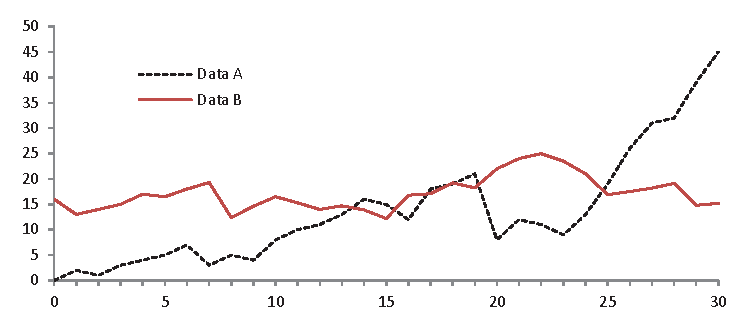
\includegraphics[width=\textwidth]{fig1.eps}
\caption{A figure caption is always placed below the illustration.
Please note that short captions are centered, while long ones are
justified by the macro package automatically.} \label{fig1}
\end{figure}

\begin{theorem}
This is a sample theorem. The run-in heading is set in bold, while
the following text appears in italics. Definitions, lemmas,
propositions, and corollaries are styled the same way.
\end{theorem}
%
% the environments 'definition', 'lemma', 'proposition', 'corollary',
% 'remark', and 'example' are defined in the LLNCS documentclass as well.
%
\begin{proof}
Proofs, examples, and remarks have the initial word in italics,
while the following text appears in normal font.
\end{proof}
For citations of references, we prefer the use of square brackets
and consecutive numbers. Citations using labels or the author/year
convention are also acceptable. The following bibliography provides
a sample reference list with entries for journal
articles~\cite{ref_article1}, an LNCS chapter~\cite{ref_lncs1}, a
book~\cite{ref_book1}, proceedings without editors~\cite{ref_proc1},
and a homepage~\cite{ref_url1}. Multiple citations are grouped
\cite{ref_article1,ref_lncs1,ref_book1},
\cite{ref_article1,ref_book1,ref_proc1,ref_url1}.
% TODO: Credits

%\begin{credits}
%  \subsubsection{\ackname} A bold run-in heading in small font size at the end of the paper is
%  used for general acknowledgments, for example: This study was funded
%  by X (grant number Y).
%  
%  \subsubsection{\discintname}
%  It is now necessary to declare any competing interests or to specifically
%  state that the authors have no competing interests. Please place the
%  statement with a bold run-in heading in small font size beneath the
%  (optional) acknowledgments\footnote{If EquinOCS, our proceedings submission
%  system, is used, then the disclaimer can be provided directly in the system.},
%  for example: The authors have no competing interests to declare that are
%  relevant to the content of this article. Or: Author A has received research
%  grants from Company W. Author B has received a speaker honorarium from
%  Company X and owns stock in Company Y. Author C is a member of committee Z.
%\end{credits}
%
% ---- Bibliography ----
%
% BibTeX users should specify bibliography style 'splncs04'.
% References will then be sorted and formatted in the correct style.
%
% \bibliographystyle{splncs04}
% \bibliography{mybibliography}
%
% \begin{thebibliography}{8}
  % \bibitem{ref_article1}
  % Author, F.: Article title. Journal \textbf{2}(5), 99--110 (2016)
  % 
  % \bibitem{ref_lncs1}
  % Author, F., Author, S.: Title of a proceedings paper. In: Editor,
  % F., Editor, S. (eds.) CONFERENCE 2016, LNCS, vol. 9999, pp. 1--13.
  % Springer, Heidelberg (2016). \doi{10.10007/1234567890}
  % 
  % \bibitem{ref_book1}
  % Author, F., Author, S., Author, T.: Book title. 2nd edn. Publisher,
  % Location (1999)
  % 
  % \bibitem{ref_proc1}
  % Author, A.-B.: Contribution title. In: 9th International Proceedings
  % on Proceedings, pp. 1--2. Publisher, Location (2010)
  % 
  % \bibitem{ref_url1}
  % LNCS Homepage, \url{http://www.springer.com/lncs}, last accessed 2023/10/25
% \end{thebibliography}

\bibliographystyle{splncs04}
\bibliography{references}

% TODO: Cite properly, Upper case issue

\end{document}
